\documentclass{article}

\date{19 septembre 2024}
\usepackage[nb-sem=1, auteurs={George Ober, Félix Rondeau}]{../kholles}

%\pgfplotsset{compat=1.17}

\begin{document}

\maketitle


\allowdisplaybreaks[4]
\begin{question_kholle}{Preuve formelle de la somme des entiers et des termes d'une suite géométrique}
  \begin{itemize}[label=$\lozenge$]
    \item Soit $n \in \mathbb{N}$ fixé quelconque. Posons $$S_{n} = \sum_{k=0}^{n}k$$
          En posant la symétrie d'indice $i = n-k$, on a aussi
          $$
            S_{n}= \sum_{i=0}^{n}(n-i)=\sum_{i=0}^{n}n - \sum_{i=0}^{n}i=(n \times \mathrm{card}[ \! [ 0, n ] \!]) - \sum_{i=0}^{n} i
          $$
          Or, puisque $\mathrm{card}[ \! [ 0, n ] \!] = n + 1$ et que $\sum_{i=0}^{n} i = S_{n}$
          $$
            S_{n} = n \times (n+1) + S_{n}
          $$
          Donc
          $$
            S_{n} = \frac{n(n+1)}{2}
          $$
    \item Soient $q \in \mathbb{R}$ , $k \in \mathbb{N}$ fixés quelconques.
          \begin{itemize}[label=$\star$]
            \item Si $q = 1$,
                  $$
                    \sum_{i=0}^{k}q^{i} = \sum_{i=0}^{k}1 = k+1
                  $$
            \item Sinon, avec l'identité algébrique, on a
                  $$
                    q^{k+1}-1^{k+1} = (q-1) \sum_{i=0}^{k}q^{i}\times 1^{k-i}
                  $$
                  Ainsi, puisque $q \neq 1$ on a, par multiplication par $(q-1)^{-1}$
                  $$
                    \sum_{i=0}^{k}q^{i} = \frac{q^{k+1}-1}{q-1}
                  $$
                  Nous avons donc établi que
                  $$
                    \sum_{i=0}^{k} q^{i} = \left\{ \begin{array}{ll}
                      \displaystyle\frac{1-q^{k+1}}{1-q} & \text{ si } q \neq 1 \\
                      k + 1                              & \text{ sinon}
                    \end{array}\right.
                  $$
          \end{itemize}
  \end{itemize}
\end{question_kholle}

\pagebreak
\begin{question_kholle}{Preuve de la factorisation de $a^n - b^n$ puis de celle de $a^{2m+1} + b^{2m+1} $}
  Soient $(a,b)\in\C^2$ et $n\in\N$ fixés quelconques.

  \begin{align*}
    (a-b)\sum_{k=0}^{m-1}a^{k}b^{m-1-k}
     & =a \sum_{k=0}^{m-1}a^{k}b^{m-1-k} -b \sum_{k=0}^{m-1}a^{k}b^{m-1-k} \\
     & = \sum_{k=0}^{m-1}a^{k+1}b^{m-1-k} - \sum_{k=0}^{m-1}a^{k}b^{m-k}   \\
  \end{align*}
  Si bien qu'en posant le changement d'indice $j = k + 1$ on reconnait le téléscopage.
  $$
    \sum_{j=1}^{m}a^{j}b^{m-j} - \sum_{k=0}^{m-1}a^{k}b^{m-k} = a^{m} - b ^{m}
  $$
  Soit $m$ un entier naturel fixé quelconque. En particularisant la relation pour $n\leftarrow 2m+1$ et $b\leftarrow (-b)$, on obtient
  \begin{align*}
    a^{2m+1} - (-b)^{2m+1} = a^{2m+1} + b^{2m+1} & = (a-(-b))\sum_{k=0}^{2m}{a^k (-b)^{2m-k}}             \\
                                                 & = (a+b)\sum_{k=0}^{2m}{a^k (-1)^{2m}(-1)^{-k}b^{2m-k}} \\
                                                 & = (a+b)\sum_{k=0}^{2m}{(-1)^k a^k b^{2n-k}}
  \end{align*}
\end{question_kholle}

\begin{question_kholle}[{Pour tout $(a, b) \in \C^2$, $n \in \N$: $$(a+b)^{n} = \sum_{k=0}^{n}\binom n k a^{k} b^{n-k}$$}]{Preuve de la formule du binôme de Newton}
  Soient $(a, b) \in \mathbb{C}^{2}$ fixés quelconques.
  Posons le prédicat $\prop(\cdot)$ défini pour tout $n \in \mathbb{N}$ par
  $$
    \prop(n): (a+b)^{n} = \sum_{k=0}^{n}\binom n k a^{k} b^{n-k}
  $$
  \begin{itemize}[label=$\star$]
    \item Initialisation, $n \leftarrow 0$
          D'une part $(a+b)^{0} = 0$, même si les deux sont nuls (par convention $0^{0} =0$)
          D'autre part
          $$
            \sum_{k=0}^{0}\binom 0 k a^{k}b^{n-k} = \binom 0 0 a^{0} b^{0} = 0
          $$
          Donc $\prop(0)$ est vérifée.

    \item Soit $n \in \mathbb{N}$ fixé quelconque tel que $\prop(n)$ est vraie

          \begin{align*}
            (a+b)^{n+1}                                 & = (a+b)\times(a+b)^{n}                                                                                        \\
                                                        & = (a+b) \times \sum_{k=0}^{n}\binom n k a^{k} b^{n-k}                                                         \\
                                                        & = a\sum_{k=0}^{n}\binom n k a^{k} b^{n-k} + b\sum_{k=0}^{n}\binom n k a^{k} b^{n-k}                           \\
                                                        & = \sum_{k=0}^{n}\binom n k a^{k+1} b^{n-k} + \sum_{k=0}^{n}\binom n k a^{k} b^{n+1-k}                         \\
                                                        & = \sum_{j=1}^{n+1}\binom n {j-1} a^{j} b^{n+1-j} + \sum_{k=0}^{n}\binom n k a^{k} b^{n+1-k}                   \\
            (\text{en posant } j = k + 1)               & = a^{n+1} + \sum_{j=1}^{n}\binom n {j-1} a^{j} b^{n+1-j} + \sum_{k=1}^{n}\binom n k a^{k} b^{n+1-k} + b^{n+1} \\
                                                        & = a^{n+1} + \left( \sum_{k=1}^{n} \left(\binom n {k-1} + \binom n k \right) a^{k} b^{n+1-k} \right) + b^{n+1} \\
            (\text{en utilisant la relation de Pascal}) & = a^{n+1} + \sum_{k=1}^{n} \binom {n+1} k a^{k} b^{n+1-k} + b^{n+1}                                           \\
                                                        & =\sum_{k=0}^{n+1} \binom {n+1} k a^{k} b^{n+1-k}
          \end{align*}

          Donc $\prop(n+1)$ est vraie.
  \end{itemize}
\end{question_kholle}

\begin{question_kholle}[
  {$$\left( \sum_{k=1}^{n}x_{k} \right)^{2} = \sum_{\substack{1\leqslant k \leqslant n\\ 1 \leqslant j \leqslant n}} x_{k}x_{j} = 2 \sum_{1\leqslant k < j \leqslant n} x_{k}x_{j}+\sum_{k=1}^{n}x_{i}^{2}$$}
  ]{Développement d'une somme}

  \begin{align*}
    \left( \sum_{k=0}^{n}x_{k} \right)^{2}
     & = \left( \sum_{k=1}^{n} x_{k} \right) \times \left( \sum_{j=1}^{n} x_{j} \right) \\
     & = \sum_{k=1}^{n}\left[ x_{k} \times \sum_{j=1}^{n}x_{j} \right]                  \\
     & = \sum_{k=1}^{n}\left( \sum_{j=1}^{n} x_{k}\times x_{j} \right)                  \\
     & = \sum_{\substack{1\leqslant k \leqslant n                                       \\ 1 \leqslant j \leqslant n}} x_{k}x_{j}
  \end{align*}


  On peut aussi séparer cette somme

  \begin{align*}
    \sum_{\substack{1\leqslant k \leqslant n                                                                  \\ 1 \leqslant j \leqslant n}} x_{k}x_{j}
                                                                                                          & =
    \sum_{\substack{1\leqslant k \leqslant n                                                                  \\ 1 \leqslant j \leqslant n \\ k<j}} x_{k}x_{j} &+
    \sum_{\substack{1\leqslant k \leqslant n                                                                  \\ 1 \leqslant j \leqslant n\\k=j}} x_{k}x_{j} &+
    \sum_{\substack{1\leqslant k \leqslant n                                                                  \\ 1 \leqslant j \leqslant n\\k>j}} x_{k}x_{j}\\
                                                                                                          & =
    \sum_{\substack{1\leqslant k \leqslant n                                                                  \\ 1 \leqslant j \leqslant n \\ k<j}} x_{k}x_{j} & +
    \underbrace{ \sum_{k=1}^{n}x_{k}^{2} }_{ \text{somme sur les indices }(k,j) \text{ tels que } k = j } & +
    \sum_{\substack{1\leqslant k \leqslant n                                                                  \\ 1 \leqslant j \leqslant n\\k>j}} x_{k}x_{j}
  \end{align*}

  On remarque aussi qu'en permutant les indices des deux sommes (les variables sont muettes)
  $$
    \sum_{\substack{1\leqslant k \leqslant n\\ 1 \leqslant j \leqslant n \\ k<j}} x_{k}x_{j} = \sum_{\substack{1\leqslant j \leqslant n\\ 1 \leqslant k \leqslant n\\j<k}} x_{j}x_{k}
  $$
  Qui, par commutativité du produit dans $\mathbb{C}$ nous donne cette égalité
  $$
    \sum_{\substack{1\leqslant k \leqslant n\\ 1 \leqslant j \leqslant n \\ k<j}} x_{k}x_{j} =
    \sum_{\substack{1\leqslant k \leqslant n\\ 1 \leqslant j \leqslant n\\k>j}} x_{k}x_{j}
  $$
  On a donc bien l'identité attendue :
  $$
    \sum_{\substack{1\leqslant k \leqslant n\\ 1 \leqslant j \leqslant n}} x_{k}x_{j} = 2 \sum_{\substack{1\leqslant k \leqslant n\\ 1 \leqslant j \leqslant n \\ k<j}} x_{k}x_{j} +
    \sum_{k=1}^{n}x_{k}^{2}
  $$
\end{question_kholle}

\begin{question_kholle}{Montrer que tout entier $n > 2$ admet un diviseur premier}
  Raisonnons par récurrence forte avec la propriété $\prop(\cdot)$ définie pour tout $n > 2$ par
  $$
    \prop(n) : \frquote{\forall k \in [ \! [ 2, n ] \!], k \text{ admet un diviseur premier}}
  $$
  \begin{itemize}
    \item Initialisation: $n \leftarrow 2$

          Soit $k \in [ \! [ 2, 2 ] \!]$ fixé quelconque. Nécéssairement, $k = 2$.
          or, $2$ admet $2$ pour diviseur premier.

          Donc $\forall k \in [ \! [ 2, 2 ] \!], k \text{ admet un diviseur premier}$, ce qui prouve $\prop(2)$.

    \item Hérédité: Soit $n \in \mathbb{N} \setminus \{ 1, 0 \}$ fixé quelconque tel que $\prop(n)$ est vraie.

          Pour montrer $\prop(n+1)$, il nous faudra montrer que $\forall k \in [ \! [ 2, n+1 ] \!], k \text{ admet un diviseur premier }$

          Soit $k \in [ \! [ 2, n+1 ] \!]$ fixé quelconque.
          \begin{itemize}[label=$\star$]
            \item    Si $k \in [ \! [ 2, n ] \!]$, alors la véracité de $\prop(n)$ nous permet de conclure, et de dire que k admet un diviseur premier.

            \item Sinon $k = n + 1$
                  \begin{itemize}[label=$\lozenge$]
                    \item Si $n+1$ est premier, alors il admet $k$ comme diviseur premier
                    \item Sinon, $\exists d \in [ \! [ 2, n ] \! ]: d \mid n+1$

                          Mais, puisque $d \in [ \! [ 2, n ] \! ]$, la véracité de $\prop(n)$ nous permet d'affirmer que $d$ admet un diviseur premier $p$. Donc par transitivité de la relation de divisibilité $$(p \mid d \text{ et } d \mid n) \implies p \mid n$$
                  \end{itemize}
          \end{itemize}
  \end{itemize}
\end{question_kholle}

\begin{question_kholle}{Montrer par récurrence qu'une fonction polynomiale à coefficients réels est nulle si et seulement si tous ses coefficients sont nuls}
  Considérons le prédicat $\prop(\cdot)$ défini pour tout $n \in \mathbb{N}$
  $$
    \prop(n) : \text{toute fonction polynômiale identiquement nulle sur }\mathbb{R} \text{ a tous ses coefficients nuls}
  $$
  Autrement dit
  $$
    \prop(n) : \forall(a_{0}, \dots ,a_{n}) \in \mathbb{R}^{n+1}\left( \forall x \in \mathbb{R}, \sum_{k=0}^{n}a_{k}x^{k} = 0 \right) \implies \forall k \in [ \! [ 0, n ] \!], a_{k} = 0
  $$
  \begin{itemize}[label=$\lozenge$]
    \item Pour $n \leftarrow 0$
          Soit $a_{0} \in \mathbb{R}$ fixé quelconque tel que $\forall x \in \mathbb{R}, a_{0}x^{0} = 0$ Alors $a_{0} = 0$

    \item Soit $n \in \mathbb{N}$ fixé quelconque tel que $\prop(n)$ est vraie
          Soient $(a_{0},\dots, a_{n+1}) \in \mathbb{R}^{n+2}$
          Posons $Q(x) = \sum_{k=0}^{n+1}a_{k}x^{k}$ tel que $\forall x \in \mathbb{R}, Q(x) = 0$
          D'une part
          $$
            \forall x \in \R, \underbrace{ Q(2x) }_{ =0 } - 2^{n+1}\underbrace{ Q(x) }_{ =0 } = 0
          $$
          D'autre part

          \begin{align*}
            \forall x \in \mathbb{R}, Q(2x) - 2^{n+1}Q(x) & = \sum_{k=0}^{n+1}a_{k}(2x)^{k}-2^{n+1}\sum_{k=0}^{n+1}a_{k}x^{k} \\
                                                          & = \sum_{k=0}^{n+1}a_{k}(2^{k}-2^{n+1})x^{k}
          \end{align*}

          Le terme d'indice $n+1$ s'annule, si bien que l'on peut écrire
          $$\forall x \in \mathbb{R}, Q(2x) - 2^{n+1}Q(x) = \sum_{k=0}^{n}a_{k}(2^{k}-2^{n+1})x^{k}$$
          Qui est une fonction polynômiale de degré $\leqslant n$, ce qui permet d'appliquer $\prop(n)$ pour $(a_{k})_{k \in[ \! [ 0, n ] \!]} \leftarrow (a_{k}(2^{k}-2^{n+1}))_{k \in[ \! [ 0, n ] \!]}$.

          Donc $\forall x \in [ \! [ 0, n ] \!]: a_{k}(2^{k}-2^{n+1}) = 0$ et puisque $2^{k}-2^{n+1} \neq 0$, on en déduit que $$\forall k \in [ \! [ 0, n ] \!], a_{k} = 0$$

          L'expression de $Q$ devient:
          $$
            \forall x \in \mathbb{R}, \underbrace{ \sum_{k=0}^{n}a_{k}x^{k} }_{ =0 }+ a_{n+1}x^{n+1} = 0
          $$
          Donc en particularisant pour $x\leftarrow 1$, on en déduit que $a_{n+1} = 0$

          Donc $\prop(n+1)$ est vraie.
  \end{itemize}
\end{question_kholle}

\begin{question_kholle}{Montrer par analyse/synthèse qu'une fonction réelle d'une variable réelle s'écrit de manière unique comme somme d'une fonction paire et d'une fonction impaire}
  Soit $f \in \mathcal{F}(\mathbb{R}, \mathbb{R})$ fixée quelconque.
  \begin{itemize}[label=$\lozenge$]


    \item \underline{Analyse}:
          Supposons que $f : \mathbb{R} \to \mathbb{R}$ se décompose de manière unique en $f = g+h$ avec $g$ paire et $h$ impaire (i.e. $\forall x \in \mathbb{R}, g(-x)= g(x)$ et $h(-x)= -h(x)$).
          Soit $x \in \mathbb{R}$ fixé quelconque
          Calculons $f(-x)$:
          $$f(-x) = g(-x) + h(-x) = g(x) -h(x)$$
          Par demi somme, nous avons donc
          $$
            \left\{ \begin{array}{ll}
              2g(x)  = f(x)+f(-x) \\
              2h(x) = f(x)-f(-x)
            \end{array}\right.
          $$
          Ainsi, si une telle décomposition existe, c'est
          $$
            \left\{ \begin{array}{ll}
              g : x \mapsto \frac{f(x)+f(-x)}{2} \\
              h : x \mapsto \frac{f(x)-f(-x)}{2}
            \end{array}\right.
          $$

    \item \underline{Synthèse}:
          Posons

          \begin{align}
            g\left|\begin{array}{ll} \mathbb{R} &\to \mathbb{R} \\ x &\mapsto \frac{f(x)+f(-x)}{2} \end{array}\right.
            \text{ et } h \left|\begin{array}{ll} \mathbb{R} &\to \mathbb{R} \\ x &\mapsto \frac{f(x)-f(-x)}{2} \end{array}\right.
          \end{align}


          Remarquons, d'une part que:
          $$
            \forall x \in \mathbb{R}, g(x)+h(x) = \frac{f(x)+f(-x)}{2} + \frac{f(x)-f(-x)}{2} = f(x)
          $$
          Vérifions si les fonctions $g$ et $h$ vérifient les conditions de parité:
          $$
            \forall x \in \mathbb{R}, g(-x) = \frac{f(-x)+f(-(-x))}{2}= \frac{f(x)+f(-x)}{2} = g(x) \text{ ainsi } g \text{ est paire.}
          $$
          $$
            \forall x \in \mathbb{R}, h(-x) = \frac{f(-x)-f(-(-x))}{2} = -\frac{f(x)-f(-x)}{2} = -h(x) \text{ ainsi } h \text{ est impaire}
          $$
  \end{itemize}
\end{question_kholle}

\begin{question_kholle}[]{Illustration graphique de certaines identités trigonométriques}
  \hfill\\
  \begin{minipage}{0.5\textwidth}
      
    \begin{figure}[H]
      \centering
    
      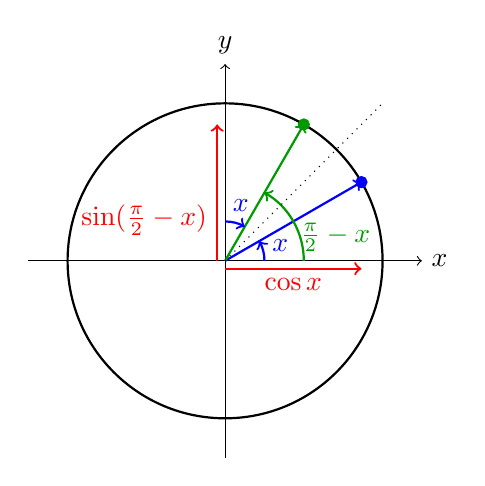
\begin{tikzpicture}
        
        \draw[thick] (0,0) circle (2);
        
        
        \draw[->] (-2.5,0) -- (2.5,0) node[right] {$x$};
        \draw[->] (0,-2.5) -- (0,2.5) node[above] {$y$};
        

        \def\angle{30}
        \def\compAngle{60}
        

        \draw[thick, ->, blue] (0,0) -- ({2*cos(\angle)}, {2*sin(\angle)});

        

        \draw[thick, ->, green!60!black] (0,0) -- ({2*sin(\angle)}, {2*cos(\angle)});

        
        
        \draw[thick,->, blue] (0.5,0) arc (0:\angle:0.5);
        \node[blue] at (0.7,0.2) {$x$};
        
        \draw[->, thick, green!60!black] (1,0) arc (0:\compAngle:1);
        \node[green!60!black] at (1.4,0.3) {$\frac \pi 2 - x$};
        
        \draw[thick,->,  blue] (0,0.5) arc (90:\compAngle:0.5);
        \node[blue] at (0.2,0.7) {$x$};
        
        \filldraw[blue] ({2*cos(\angle)}, {2*sin(\angle)}) circle (2pt);
        \filldraw[green!60!black] ({2*sin(\angle)}, {2*cos(\angle)}) circle (2pt);
        
        \draw[thick, ->, red] (-0.1, 0) -- (-0.1, {2*cos(\angle)}) node[pos=0.3, left]{$\sin(\frac \pi 2 - x)$};
        \draw[thick, ->, red] (0, -0.1) -- ({2*cos(\angle)}, -0.1) node[pos=0.5, below]{$\cos x$};

        \draw[dotted] (0, 0) -- (2, 2);

      \end{tikzpicture}
      \caption{Illustration de $\sin (\frac \pi 2 -  x) = \cos x$. On retrouve l'égalité par réflexion sur la première bissectrice.}
    \end{figure}
  \end{minipage}
  \begin{minipage}{0.5\textwidth}
      
    \begin{figure}[H]
      \centering
    
      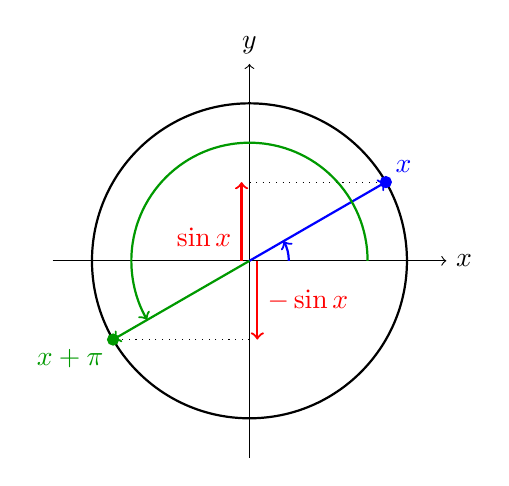
\begin{tikzpicture}

        \draw[thick] (0,0) circle (2);
        

        \draw[->] (-2.5,0) -- (2.5,0) node[right] {$x$};
        \draw[->] (0,-2.5) -- (0,2.5) node[above] {$y$};
        

        \def\angle{30} 
        \def\compAngle{210}
        

        \draw[thick, ->, blue] (0,0) -- ({2*cos(\angle)}, {2*sin(\angle)});

        

        \draw[thick, ->, green!60!black] (0,0) -- ({-2*cos(\angle)}, {-2*sin(\angle)});

        
        
        \draw[thick,->, blue] (0.5,0) arc (0:\angle:0.5);
        
        \draw[dotted] (0, {2*sin(\angle)}) -- ({2*cos(\angle)}, {2*sin(\angle)});
        \draw[dotted] (0, {-2*sin(\angle)}) -- ({-2*cos(\angle)}, {-2*sin(\angle)});
        
        \draw[->, thick, green!60!black] (1.5,0) arc (0:\compAngle:1.5);
        
        
        
        
        \filldraw[blue] ({2*cos(\angle)}, {2*sin(\angle)}) circle (2pt) node[above right] {$x$};
        \filldraw[green!60!black] ({-2*cos(\angle)}, {-2*sin(\angle)}) circle (2pt)node[below left] {$x + \pi$};
        
        \draw[thick, ->, red] (-0.1, 0) -- (-0.1, {2*sin(\angle)}) node[pos=0.3, left]{$\sin x$};
        \draw[thick, ->, red] (0.1, 0) -- (0.1, -{2*sin(\angle)}) node[pos=0.5, right]{$-\sin x$};

      \end{tikzpicture}
      \caption{Illustration de $\sin (x + \pi) = - \sin x$. On retrouve l'égalité par symétrie centrale.}
    \end{figure}
  \end{minipage}
  \begin{minipage}{0.5\textwidth}
      
    \begin{figure}[H]
      \centering
    
      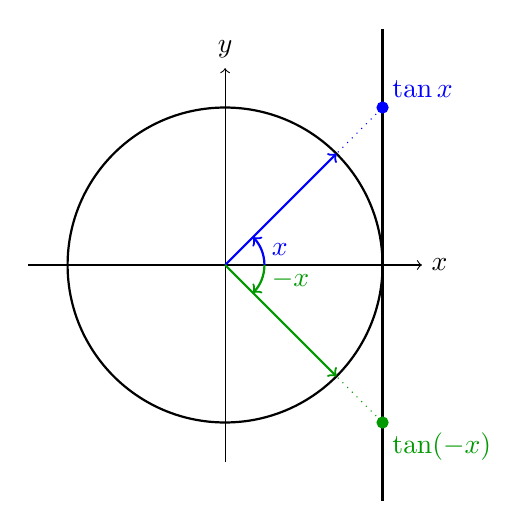
\begin{tikzpicture}

        \draw[thick] (0,0) circle (2);
        

        \draw[->] (-2.5,0) -- (2.5,0) node[right] {$x$};
        \draw[->] (0,-2.5) -- (0,2.5) node[above] {$y$};
        \draw[thick] (2, 3) -- (2, -3);

        \def\angle{45}
        \def\compAngle{-45}
        

        \draw[dotted, blue] (0,0) -- ({2}, {2*tan(\angle)});
        \draw[thick, ->, blue] (0,0) -- ({2*cos(\angle)}, {2*sin(\angle)});
        
        
        
        \draw[dotted, green!60!black] (0,0) -- ({2}, {-2*tan(\angle)});
        \draw[thick, ->, green!60!black] (0,0) -- ({2*cos(\angle)}, {-2*sin(\angle)});

        
        
        \draw[thick,->, blue] (0.5,0) arc (0:\angle:0.5) node[pos=0.5, right] {$x$};
        
        
        \draw[->, thick, green!60!black] (0.5,0) arc (0:\compAngle:0.5) node[pos=0.5, right] {$-x$};
        
        
        
        
        \filldraw[blue] (2, {2*tan(\angle)}) circle (2pt) node[above right] {$\tan x$};
        \filldraw[green!60!black] (2, {-2*tan(\angle)}) circle (2pt) node[below right] {$\tan (-x)$};
        
        

      \end{tikzpicture}
      \caption{Illustration de $\tan (-x) = - \tan x$. On retrouve l'égalité par réflexion sur l'axe des abscisses.}
    \end{figure}
  \end{minipage}
  \begin{minipage}{0.5\textwidth}
      
    \begin{figure}[H]
      \centering
    
      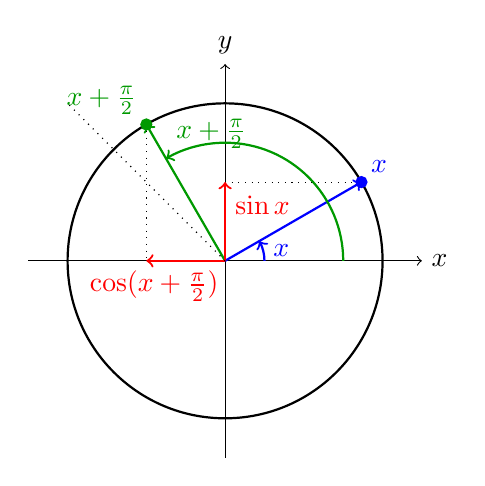
\begin{tikzpicture}
        
        \draw[thick] (0,0) circle (2);
        
        
        \draw[->] (-2.5,0) -- (2.5,0) node[right] {$x$};
        \draw[->] (0,-2.5) -- (0,2.5) node[above] {$y$};
        

        \def\angle{30} 
        \def\compAngle{120}
        

        \draw[thick, ->, blue] (0,0) -- ({2*cos(\angle)}, {2*sin(\angle)});

        

        \draw[thick, ->, green!60!black] (0,0) -- ({2*cos(\compAngle)}, {2*sin(\compAngle)});

        
        
        \draw[thick,->, blue] (0.5,0) arc (0:\angle:0.5) node[pos=0.5, right] {$x$};
        
        \draw[dotted] (0, {2*sin(\angle)}) -- ({2*cos(\angle)}, {2*sin(\angle)});
        \draw[dotted] ({2*cos(\compAngle)}, {2*sin(\compAngle)}) -- ({2*cos(\compAngle)}, 0);
        
        \draw[->, thick, green!60!black] (1.5,0) arc (0:\compAngle:1.5) node[pos=1, above right] {$x + \frac \pi 2$};
        
        
        
        
        \filldraw[blue] ({2*cos(\angle)}, {2*sin(\angle)}) circle (2pt) node[above right] {$x$};
        \filldraw[green!60!black] ({2*cos(\compAngle)}, {2*sin(\compAngle)}) circle (2pt)node[above left] {$x + \frac \pi 2$};
        
        \draw[thick, ->, red] (0, 0) -- (0, {2*sin(\angle)}) node[pos=0.7, right]{$\sin x$};
        \draw[thick, ->, red] (0, 0) -- ({2*cos(\compAngle)},0) node[pos=0.9, below]{$\cos (x + \frac \pi 2)$};
        
        \draw[dotted] (0, 0) -- (-2, 2);

      \end{tikzpicture}
      \caption{Illustration de $\cos (x + \frac \pi 2) = - \sin x$. On retrouve l'égalité par réflexion sur la deuxième bissectrice.}
    \end{figure}
  \end{minipage}
\end{question_kholle}

\begin{question_kholle}{Technique de résolution des équations trigonométriques du type $A \cos x + B \sin x = C$}
  Étudions l'équation d'inconnue $x$

  $$
    A \cos x + B \sin x = C
  $$
  \begin{itemize}[label=$\star$]
    \item Si $A = 0$ et $B = 0$
          \begin{itemize}[label=$\lozenge$]
            \item Si $C = 0$ l'équation admet $\mathbb{R}$ pour ensemble de solutions
            \item Sinon, l'équation n'admet pas de solutions
          \end{itemize}
    \item Sinon,

          Factorisons par $\sqrt{ A^{2}+B^{2} }$ (ce qui a un sens car $(A, B) \neq (0, 0) \implies \sqrt{ A^{2}+ B^{2} } \neq 0$)

          $$
            \frac{A}{\sqrt{ A^{2}+B^{2} }}\cos x + \frac{B}{\sqrt{ A^{2}+B^{2} }} \sin x = \frac{C}{ \sqrt{ A^{2}+B^{2} }}
          $$
          Le nombre complexe $\frac{A}{\sqrt{ A^{2}+B^{2}} }+i \frac{B}{\sqrt{ A^{2} +B^{2}}}$ est de module $1$, donc $\exists \varphi \in \mathbb{R}$ tel que

          $$
            e^{i\varphi} = \underbrace{ \frac{A}{\sqrt{ A^{2}+B^{2}} } }_{ \cos \varphi }+i \underbrace{ \frac{B}{\sqrt{ A^{2} +B^{2}}} }_{ \sin \varphi }
          $$

          Ainsi,
          $$
            (\cos \varphi \cos x-\sin \varphi \sin x) = \frac{C}{ \sqrt{ A^{2}+B^{2} }}
          $$
          donc
          $$
            \cos(\varphi+x) = \frac{C}{\sqrt{ A^{2}+B^{2} }}
          $$
          \begin{itemize}[label=$\lozenge$]
            \item Si $\displaystyle \frac{C}{\sqrt{ A^{2}+B^{2} }}\leqslant 1$

                  \begin{align*}
                    \cos(\varphi+x) = \frac{C}{\sqrt{ A^{2}+B^{2} }} & \iff
                    \left\{ \begin{array}{ll}
                              \phi + x \equiv \arccos\frac{C}{\sqrt{ A^{2}+B^{2} }}  [2\pi] \\
                              \text{ou}                                                     \\
                              \phi + x \equiv - \arccos\frac{C}{\sqrt{ A^{2}+B^{2} }} [2\pi]
                            \end{array}\right.                                                                                                                                                                                                 \\
                                                                     & \iff x \in \begin{array}{ll}\left\{ \arccos \frac{C}{\sqrt{ A^{2}+B^{2} }} + 2k\pi \mid k \in \mathbb{Z} \right\} \\ \cup \\ \left\{- \arccos \frac{C}{\sqrt{ A^{2}+B^{2} }} + 2k\pi \mid k \in \mathbb{Z} \right\}
                                                                                  \end{array}
                  \end{align*}


            \item Sinon, l'équation n'admet aucune solution
          \end{itemize}
  \end{itemize}
\end{question_kholle}

\begin{question_kholle}{Étude complète de la fonction tangente, tracé du graphe et en déduire celui de cotangente.}
\end{question_kholle}

\begin{question_kholle}{Expression de $\sin \theta$, $\cos \theta$, $\tan \theta$ en fonction de $\tan \frac \theta 2$}
  Soit $\theta \in \mathbb{R} \setminus \pi \mathbb{Z}$.
  Posons $\displaystyle u = \tan \frac{\theta}{2}$
  \begin{itemize}[label=$\lozenge$]
    \item $\displaystyle \tan \theta = \frac{2u}{1-u^{2}}$

          En utilisant la formule classique de trigonométrie

          $$\tan (a+b) = \frac{\tan a+\tan b}{1-\tan a\tan b}$$

          On obtient, avec $(a,b) \leftarrow (\frac{\theta}{2}, \frac{\theta}{2})$
          $$
            \tan \theta = \frac{2 \tan \frac{\theta}{2}}{1-\tan ^{2} \frac{\theta}{2}}=\frac{2u}{1-u^{2}}
          $$


    \item $\displaystyle \cos \theta = \frac{1-u^{2}}{1+u^{2}}$
          \begin{align*}
            \cos \theta & = 2\cos ^{2} \frac{\theta}{2} -1             \\
                        & = \frac{2}{1+\tan ^{2} \frac{\theta}{2}} - 1 \\
                        & = \frac{2}{1+u^{2}}-1                        \\
                        & = \frac{1-u^{2}}{1+u^{2}}
          \end{align*}

    \item $\displaystyle \sin \theta \frac{2u}{1+u^{2}}$

          \begin{align*}
            \sin \theta & = \cos \theta \tan \theta                           \\
                        & = \frac{1-u^{2}}{1+u^{2}} \times \frac{2u}{1-u^{2}} \\
                        & = \frac{2u}{1+u^{2}}
          \end{align*}
  \end{itemize}
\end{question_kholle}

\begin{question_kholle}{Preuve des formules du type $\cos p + \cos q = \dots$}
  Partons des formules d'addition

  $$
    \cos (a+b) = \cos a\cos b-\sin a\sin b\\
  $$
  $$
    \cos (a-b) = \cos a\cos b+\sin a\sin b
  $$

  \begin{align*}
    \cos(a+b) + \cos (a-b) = 2\cos a\cos b
    \tag{$\spadesuit$}\label{S1:Q12:1}
  \end{align*}


  Si bien qu'en posant
  $$
    \left\{ \begin{array}{ll}
      p = a+b \\
      q= a-b
    \end{array}\right.
    \iff
    \left\{ \begin{array}{ll}
      a = \frac{p+q}{2} \\
      b= \frac{p-q}{2}
    \end{array}\right.
  $$
  D'où, en injectant dans \eqref{S1:Q12:1}
  $$
    \cos p + \cos q = 2\cos \frac{p+q}{2} \cos \frac{p-q}{2}
  $$

\end{question_kholle}
\end{document}
